\documentclass[10pt]{beamer}
\usepackage[utf8]{inputenc}
\usepackage[T1]{fontenc}
\usepackage{amsmath,amssymb}
\usepackage{bm}
\usepackage{tikz}
\usetikzlibrary{arrows.meta, positioning, shapes, decorations.pathmorphing}
\usepackage{listings}
\usepackage{xcolor}
\usepackage{booktabs}
\usepackage{hyperref}
\usepackage{geometry}
\geometry{margin=1cm}

\usetheme{Madrid}
\usecolortheme{seahorse}

\definecolor{codegreen}{rgb}{0,0.6,0}
\definecolor{codegray}{rgb}{0.5,0.5,0.5}
\definecolor{codepurple}{rgb}{0.58,0,0.82}
\definecolor{backcolour}{rgb}{0.95,0.95,0.92}
\definecolor{seagreen}{RGB}{0,100,80}

\lstdefinestyle{mystyle}{
    backgroundcolor=\color{backcolour},
    commentstyle=\color{codegreen},
    keywordstyle=\color{magenta!70!black},
    numberstyle=\tiny\color{codegray},
    stringstyle=\color{codepurple},
    basicstyle=\ttfamily\footnotesize,
    breakatwhitespace=false,
    breaklines=true,
    captionpos=b,
    keepspaces=true,
    numbers=left,
    numbersep=5pt,
    showspaces=false,
    showstringspaces=false,
    showtabs=false,
    tabsize=2
}
\lstset{style=mystyle}

\title{\textbf{From the Ground Up: Derivatives $\to$ Backprop $\to$ Neural Networks}}
\subtitle{A Complete Lecture, Built in Layers}
\author{}
\institute{}
\date{}

\begin{document}

\begin{frame}[plain]
    \begin{tikzpicture}[remember picture, overlay]
        \fill[color=teal!80] (current page.south west) rectangle (current page.north east);
    \end{tikzpicture}
    \centering
    \vspace{2cm}
    {\Huge\bfseries From the Ground Up}\\[0.3cm]
    {\LARGE Derivatives $\to$ Backprop $\to$ Neural Networks}\\[0.5cm]
    {\large\color{gray} 10 Sections $\cdot$ From First Principles to Image Classification}
\end{frame}

\begin{frame}{Table of Contents}
    \tableofcontents[hideallsubsections]
\end{frame}

% ===== PART 1 =====
\section{Derivatives}

\begin{frame}{What is a Derivative?}
    \textbf{The Question:} Given $f(x)$, how should we change $x$ to make $f(x)$ smaller?
    \vspace{0.5cm}
    \textbf{The Definition:}
    \[
        f'(x) = \lim_{h \to 0} \frac{f(x+h) - f(x)}{h}
    \]
    \textit{``If I nudge $x$ by a tiny amount, how much does $f$ change, per unit of nudge?''}
    \vspace{0.5cm}
    \textbf{Examples:}
    \[
        \begin{array}{c|c|c}
            f(x) & f'(x) & \text{Meaning} \\
            \hline
            x^2 & 2x & \text{at } x=3, \text{ slope is } 6 \\
            3x+1 & 3 & \text{constant slope} \\
            \sin(x) & \cos(x) & \text{oscillates} \\
            e^x & e^x & \text{slope equals value}
        \end{array}
    \]
\end{frame}

\begin{frame}{The Linear Approximation}
    \[
        f(x + h) \approx f(x) + f'(x) \cdot h
    \]
    \textbf{``New value $\approx$ old value + (slope) $\times$ (how far I moved).''}
    This is the \textbf{only} first-order approximation matching $f$ at $x$ with correct slope.
    \vspace{0.5cm}
    \begin{tikzpicture}[scale=0.8]
        \draw[->] (-0.5,0) -- (4.5,0) node[right]{$x$};
        \draw[->] (0,-0.5) -- (0,4.5) node[above]{$f(x)$};
        \draw[smooth,domain=0:4,variable=\x,blue,thick] plot ({\x},{\x*\x/2});
        \draw[dashed,red,thick] (2,1) -- (3.5,3.25);
        \fill[blue] (2,1) circle (2pt);
        \node[blue] at (2.1,1.3){$f(x)$};
        \node[red] at (3.2,2.8){tangent};
    \end{tikzpicture}
\end{frame}

\begin{frame}{The Learning Rule}
    \[
        x_{\text{new}} = x - \eta \cdot f'(x)
    \]
    \begin{itemize}
        \item If $f'(x) > 0$: decrease $x$
        \item If $f'(x) < 0$: increase $x$
    \end{itemize}
    \textbf{The sign tells direction; the magnitude tells steepness.}
    This is gradient descent in one dimension.
\end{frame}

% ===== PART 2 =====
\section{The Chain Rule}

\begin{frame}{Compositions}
    Real functions are compositions:
    \[
        u = 3x + 1, \quad v = u^2, \quad f = v + 5
    \]
    \textbf{The Rule:}
    \[
        \frac{df}{dx} = \frac{df}{dv} \cdot \frac{dv}{du} \cdot \frac{du}{dx}
    \]
    \textbf{Intuition:} Think of each derivative as a ratio of small changes:
    \[
        \frac{\Delta f}{\Delta x} = \frac{\Delta f}{\Delta v} \cdot \frac{\Delta v}{\Delta u} \cdot \frac{\Delta u}{\Delta x}
    \]
    The intermediate differentials cancel like fractions.
\end{frame}

\begin{frame}{Concrete Example}
    With $x = 2$: $u = 7$, $du/dx = 3$; $v = 49$, $dv/du = 14$; $f = 54$, $df/dv = 1$.
    \[
        \frac{df}{dx} = 1 \cdot 14 \cdot 3 = 42
    \]
    \textbf{Check directly:} $f(x) = (3x+1)^2 + 5$, $f'(x) = 6(3x+1) = 42$. \checkmark

    \textbf{Branching:} $f = g(x) + h(x) \implies df/dx = dg/dx + dh/dx$
\end{frame}

\begin{frame}{Why This Is the Whole Game}
    Every neural network is a deeply nested composition.
    \[
        \text{Loss} = L(\text{MLP}(\text{image}))
    \]
    The chain rule lets us compute $\partial\text{Loss}/\partial\theta$ for every parameter $\theta$ by multiplying local derivatives along the path from $\theta$ to the loss.
\end{frame}

% ===== PART 3 =====
\section{Gradient Descent}

\begin{frame}{The Optimization Problem}
    We want: $\theta^* = \arg\min_\theta \; L(\theta)$
    \vspace{0.5cm}
    \textbf{The Update Rule:}
    \[
        \theta \leftarrow \theta - \eta \cdot \frac{dL}{d\theta}
    \]
    \begin{itemize}
        \item $dL/d\theta > 0$: decrease $\theta$
        \item $dL/d\theta < 0$: increase $\theta$
        \item $dL/d\theta = 0$: at a critical point
    \end{itemize}
\end{frame}

\begin{frame}{The Learning Rate $\eta$}
    \begin{tabular}{c|l}
        \toprule
        \textbf{$\eta$ too small} & Training crawls \\
        \textbf{$\eta$ too large} & Overshoot, oscillate, diverge \\
        \textbf{$\eta$ just right} & Smooth descent to a local minimum \\
        \bottomrule
    \end{tabular}
    Typical values: 0.001 to 0.1. \textbf{The single most important hyperparameter.}
\end{frame}

% ===== PART 4 =====
\section{Gradients (Many Inputs)}

\begin{frame}{From Scalar to Vector}
    When $L$ depends on many parameters $\theta = (\theta_1, \ldots, \theta_n)$:
    \[
        \nabla L = \left[\frac{\partial L}{\partial \theta_1}, \frac{\partial L}{\partial \theta_2}, \ldots, \frac{\partial L}{\partial \theta_n}\right]
    \]
    \textbf{Elementwise Update:}
    \[
        \theta_i \leftarrow \theta_i - \eta \cdot \frac{\partial L}{\partial \theta_i} \qquad \text{for every } i
    \]
\end{frame}

\begin{frame}{The Gradient Points Uphill}
    \textbf{$\nabla L$ points in the direction of steepest ascent.} So $-\nabla L$ points downhill.
    \vspace{0.5cm}
    \textbf{The Big Realization:} For millions of parameters, computing all gradients naively requires millions of forward passes.
    \textbf{Backprop computes all gradients in one backward pass.} Cost $\approx 2\times$ forward, independent of parameter count.
\end{frame}

% ===== PART 5 =====
\section{The Autograd Engine}

\begin{frame}{The Value Class}
    \begin{lstlisting}[language=Python, caption={The Value class skeleton}]
class Value:
    def __init__(self, data, _children=(), _op=''):
        self.data = data
        self.grad = 0.0
        self._backward = lambda: None
        self._prev = set(_children)
        self._op = _op
    \end{lstlisting}
    Each \texttt{Value} stores: its \textbf{data}, its \textbf{gradient}, how it was \textbf{created}, and its \textbf{\_backward} function.
\end{frame}

\begin{frame}{Local Derivatives as Code}
    \textbf{Addition:} $\partial c/\partial a = 1$, $\partial c/\partial b = 1$.
    \begin{lstlisting}[language=Python]
def __add__(self, other):
    out = Value(self.data + other.data, (self, other), '+')
    def _backward():
        self.grad  += 1.0 * out.grad
        other.grad += 1.0 * out.grad
    out._backward = _backward
    return out
    \end{lstlisting}
    \textbf{Multiplication:} $\partial c/\partial a = b$, $\partial c/\partial b = a$.
    \begin{lstlisting}[language=Python]
def __mul__(self, other):
    out = Value(self.data * other.data, (self, other), '*')
    def _backward():
        self.grad  += other.data * out.grad
        other.grad += self.data  * out.grad
    out._backward = _backward
    return out
    \end{lstlisting}
\end{frame}

\begin{frame}{Why \texttt{+=}?}
    If a value is used multiple times, gradients from all uses must \textbf{sum}.
    \[
        f = a \cdot b + a \cdot c \implies \frac{\partial f}{\partial a} = b + c
    \]
    The \texttt{+=} in both \texttt{\_backward} calls accumulates both contributions.
\end{frame}

\begin{frame}{Forward Pass Builds a Graph}
    \begin{lstlisting}[language=Python, caption={Writing expressions builds a Value DAG}]
loss = ((y_pred - y) ** 2).tanh()
    \end{lstlisting}
    Python constructs a tree of \texttt{Value} objects. The graph is the computation.
    \vspace{0.5cm}
    \begin{lstlisting}[language=Python, caption={The backward algorithm}]
def backward(self):
    topo, visited = [], set()
    def build(v):
        if v not in visited:
            visited.add(v)
            for c in v._prev: build(c)
            topo.append(v)
    build(self)
    self.grad = 1.0
    for v in reversed(topo):
        v._backward()
    \end{lstlisting}
\end{frame}

% ===== PART 6 =====
\section{Backprop}

\begin{frame}{The Setup}
    \texttt{loss} is the root. Every parameter $\theta$ is a leaf. We want $\partial\text{loss}/\partial\theta$ for every leaf.
    \vspace{0.5cm}
    \textbf{Topological Order:} Process each node \emph{after} every node that depends on it.
    \vspace{0.5cm}
    \textbf{Seeding:} $\text{loss.grad} = 1.0$ because $\partial\text{loss}/\partial\text{loss} = 1$.
\end{frame}

\begin{frame}{The Reverse Walk}
    For each node, calling \texttt{\_backward()}:
    \begin{enumerate}
        \item Reads \texttt{node.grad} (incoming gradient from all consumers).
        \item Multiplies by each local derivative.
        \item Adds results to each input's \texttt{.grad}.
    \end{enumerate}
    \textbf{This is the chain rule, evaluated in reverse, with accumulation at every node.}
\end{frame}

\begin{frame}{Why This Is Efficient}
    \textbf{Naive:} $N$ forward passes for $N$ parameters.\\
    \textbf{Backprop:} 1 forward + 1 backward $\approx 2\times$ forward, independent of parameter count.\\[4pt]
    \textbf{Backprop = Reverse-Mode Autodiff:} ``Reverse mode'' because we walk backward from the output. ``Auto-diff'' because the graph is differentiated automatically.
\end{frame}

\begin{frame}{The Full Picture}
    \begin{verbatim}
FORWARD:
  for each op in order:
      value = op(inputs)
      save inputs and value for backward

BACKWARD:
  output.grad = 1
  for each op in reverse order:
      for each input of op:
          input.grad += local_derivative(op, input) * op.output.grad
    \end{verbatim}
    That's backprop. Everything else is engineering.
\end{frame}

% ===== PART 7 =====
\section{Neural Networks}

\begin{frame}{A Neuron}
    A neuron is a small differentiable function:
    \[
        h = \tanh(w \cdot x + b)
    \]
    \begin{lstlisting}[language=Python, caption={A neuron}]
class Neuron:
    def __init__(self, nin):
        self.w = [Value(random.uniform(-1, 1) / (nin ** 0.5)) for _ in range(nin)]
        self.b = Value(0.0)

    def __call__(self, x):
        act = self.b
        for xi, wi in zip(x, self.w):
            act = act + xi * wi
        return act.tanh()

    def parameters(self):
        return self.w + [self.b]
    \end{lstlisting}
    The $1/\sqrt{n_{\text{in}}}$ init keeps the dot product's magnitude stable.
\end{frame}

\begin{frame}{Why Nonlinearity?}
    Without $\tanh$, a stack of linear layers collapses into a single linear function:
    \[
        W_2(W_1 x + b_1) + b_2 = (W_2 W_1)x + (W_2 b_1 + b_2) = Wx + b
    \]
    \textbf{No matter how deep, it's still linear.} Nonlinearity is what lets deep networks represent nonlinear functions.
\end{frame}

\begin{frame}{A Layer and The MLP}
    A layer is $n_{\text{out}}$ neurons, each seeing the same input.
    Stacking layers gives a multilayer perceptron.
    \vspace{0.5cm}
    For classification, we typically \textbf{do not} apply $\tanh$ on the last layer --- we want raw logits for softmax cross-entropy.
\end{frame}

\begin{frame}{Parameter Count}
    For $\text{MLP}(64, [32, 32, 5])$:
    \begin{table}
        \centering
        \begin{tabular}{@{}lcc@{}}
            \toprule
            Layer & Formula & Parameters \\
            \midrule
            Layer 1 & $32 \times (64+1)$ & 2080 \\
            Layer 2 & $32 \times (32+1)$ & 1056 \\
            Layer 3 & $5 \times (32+1)$ & 165 \\
            \midrule
            \textbf{Total} & & \textbf{3301} \\
            \bottomrule
        \end{tabular}
    \end{table}
    Fixed by architecture, not by dataset size.
\end{frame}

% ===== PART 8 =====
\section{The Loss}

\begin{frame}{Cross-Entropy for Classification}
    For logits $\mathbf{z}$ and target class $t$:
    \[
        \text{softmax}(\mathbf{z})_i = \frac{e^{z_i}}{\sum_j e^{z_j}}, \qquad
        \text{loss} = -\log(\text{softmax}(\mathbf{z})_t)
    \]
    The model predicts a probability distribution. Loss penalizes low probability on the correct class.
\end{frame}

\begin{frame}{Why Log + Softmax?}
    \textbf{The gradient w.r.t. the logits is beautiful:}
    \[
        \frac{\partial\text{loss}}{\partial z_i} = \text{softmax}(\mathbf{z})_i - \mathbb{1}[i = t]
    \]
    \textbf{Predicted probability $-$ one-hot target.} Well-scaled, never vanishing, never exploding.
    \textbf{Backprop derives this automatically.} We never write it by hand.

    \textbf{Why not MSE?} $\tanh$ saturates, gradients vanish when confidently wrong. MSE's gradient on probabilities is small near 0 or 1.
\end{frame}

\begin{frame}{Numerical Stability}
    $e^z$ overflows for large $z$. Subtract the max before exponentiating. Softmax is invariant to this shift.
    \begin{lstlisting}[language=Python, caption={Stable softmax cross-entropy}]
def softmax_cross_entropy(logits, target_idx):
    max_val = max(z.data for z in logits)
    shifted = [z - max_val for z in logits]
    exps = [s.exp() for s in shifted]
    total = exps[0]
    for e in exps[1:]:
        total = total + e
    probs = [e / total for e in exps]
    return -probs[target_idx].log()
    \end{lstlisting}
    Backprop handles this composition automatically.
\end{frame}

% ===== PART 9 =====
\section{The Training Process}

\begin{frame}{The Loop}
    For each batch:
    \begin{lstlisting}[language=Python, caption={Complete training step}]
# --- Forward ---
batch_loss = Value(0.0)
for img, label in batch:
    x = [Value(p) for p in img]
    logits = model(x)
    batch_loss = batch_loss + softmax_cross_entropy(logits, label)
batch_loss = batch_loss * (1.0 / BATCH_SIZE)

# --- Backward ---
for p in params: p.grad = 0.0
batch_loss.backward()

# --- Update ---
for p in params:
    p.data -= LEARNING_RATE * p.grad
    \end{lstlisting}
    \textbf{Three phases:} Forward builds the graph. Backward computes all gradients in one pass. Update steps each parameter downhill.
\end{frame}

\begin{frame}{The Three Phases}
    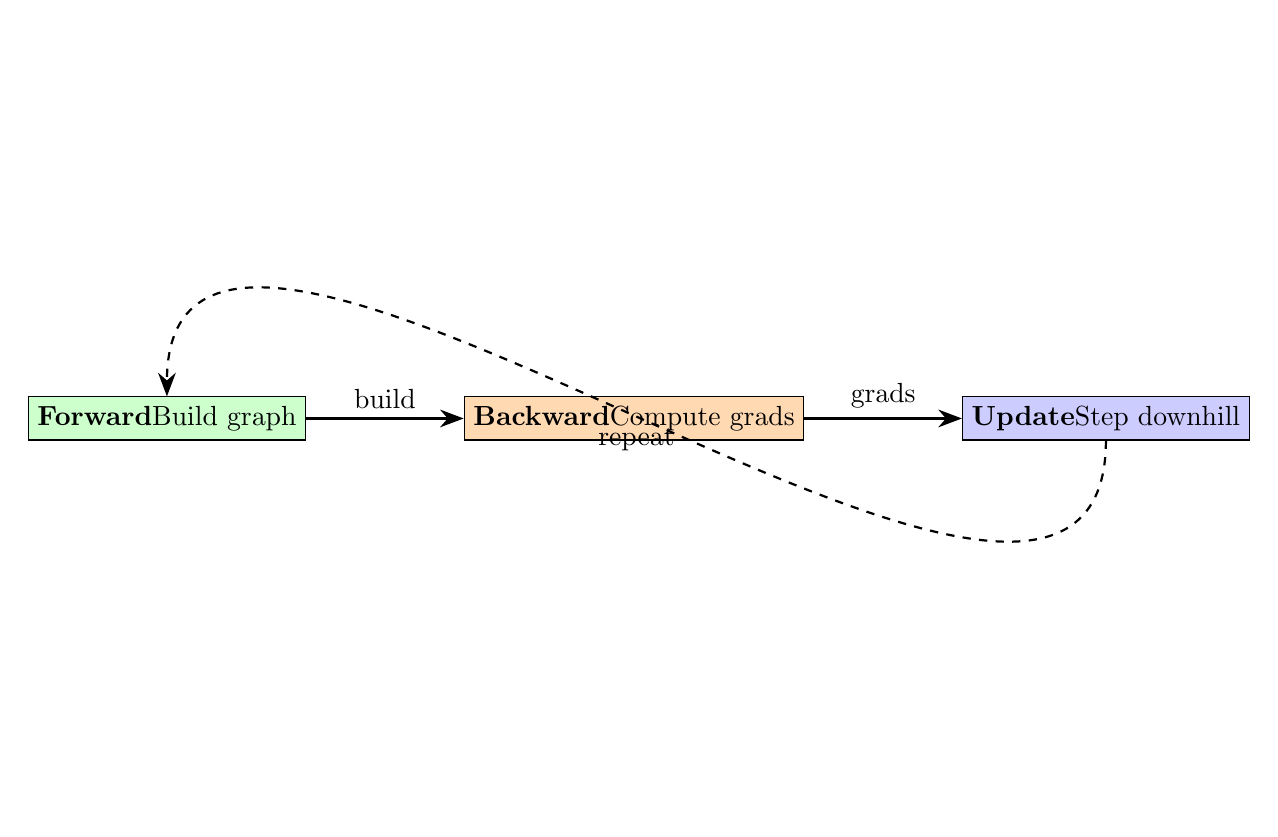
\begin{tikzpicture}[scale=0.85, node distance=2cm]
        \node[draw, fill=green!20] (fwd) {\textbf{Forward}\\[2pt]Build graph};
        \node[draw, fill=orange!30, right=of fwd] (bwd) {\textbf{Backward}\\[2pt]Compute grads};
        \node[draw, fill=blue!20, right=of bwd] (upd) {\textbf{Update}\\[2pt]Step downhill};
        \draw[-{Stealth[length=3mm]}, thick] (fwd) -- node[above]{build} (bwd);
        \draw[-{Stealth[length=3mm]}, thick] (bwd) -- node[above]{grads} (upd);
        \draw[-{Stealth[length=3mm]}, thick, dashed] (upd) to[out=270,in=90] node[below]{repeat} (fwd);
    \end{tikzpicture}
    \vspace{0.5cm}
    \textbf{Zeroing gradients:} Because \texttt{\_backward} uses \texttt{+=}. Without zeroing, training diverges.
\end{frame}

\begin{frame}{What Changes as the Model Learns}
    \textbf{Early:} loss decreases rapidly. \textbf{Middle:} useful features emerge. \textbf{Late:} slow decrease.
    \vspace{0.3cm}
    If train and test loss diverge, the model is \textbf{overfitting}. The \textbf{generalization gap} is the central tension in ML.
\end{frame}

% ===== PART 10 =====
\section{Putting It All to Work}

\begin{frame}{The Dataset}
    Synthetic $8 \times 8$ images of digits 0--4, drawn as crude strokes. Add 10\% noise. Flatten to 64 pixels.
    \vspace{0.5cm}
    \textbf{Why no convolutions?} Our goal is to understand backprop. Convs add a new op with its own backward rules, obscuring core ideas. The backprop algorithm is \textbf{identical} with or without convs.
\end{frame}

\begin{frame}{Results}
    After $\sim$40 epochs, $\eta = 0.05$:
    \[
        \begin{array}{c|c|c|c|c}
            \text{Epoch} & \text{Train Loss} & \text{Train Acc} & \text{Test Loss} & \text{Test Acc} \\
            \hline
            0  & 1.5861 & 0.281 & 1.5618 & 0.300 \\
            10 & 0.2210 & 0.881 & 0.3412 & 0.775 \\
            20 & 0.0781 & 0.963 & 0.2218 & 0.850 \\
            39 & 0.0281 & 0.991 & 0.1540 & 0.925
        \end{array}
    \]
    Train accuracy climbs to 99\%. Test accuracy plateaus at 92.5\%. The model learns.
\end{frame}

\begin{frame}{What the Model Learned}
    Reshaping first-layer weights to $8 \times 8$ reveals stroke detectors. The second layer combines these into digit-part detectors. The third layer produces class scores.
    \vspace{0.5cm}
    \textbf{This hierarchy emerges automatically from gradient descent.} We never told the model ``look for strokes.'' We told it ``minimize the loss,'' and backprop did the rest.
\end{frame}

\begin{frame}{Summary}
    \begin{center}
        \textbf{Every parameter has a derivative. Gradient descent uses these derivatives to step downhill.\\
        The chain rule tells us how to compute the derivative of a composition.\\
        Backprop is the chain rule applied systematically.\\
        A neural network is a composition of simple differentiable functions.\\
        Training is a loop: forward, backward, step.\\
        Everything else is a new differentiable op with a new local derivative.\\
        The engine never changes.}
    \end{center}
\end{frame}

\begin{frame}{Exercises}
    \textbf{1. Trace by hand.} Compute forward and backward for a 2-input neuron.
    \textbf{2. Break \texttt{+=}.} Replace with \texttt{=}. Watch gradients come out wrong.
    \textbf{3. Add ReLU.} Derive its local derivative. Compare to $\tanh$.
    \textbf{4. Remove gradient zeroing.} See training diverge.
    \textbf{5. Try MSE + $\tanh$ on classification.} Observe slow early training.
    \textbf{6. Print the graph.} Walk \texttt{\_prev} from loss. See the DAG.
    \textbf{7. Swap in NumPy.} Same math, 100$\times$ faster.
    \textbf{8. Add a conv.} Derive its backward. See the accuracy jump.
\end{frame}

\end{document}
